\chapter{Théorème de\\Pythagore et\\trigonométrie} \label{G10}

\bigskip

\begin{figure}[h]
   \centering
      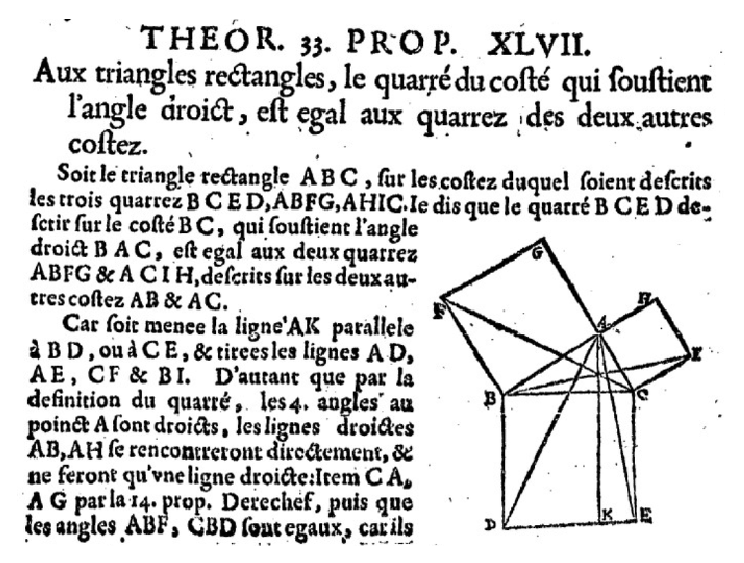
\includegraphics[height=6cm]{Geometrie/Images/G10_intro_Pythagore_Euclide}
   \caption{Les éléments d'Euclide, traduit par Didier Henrion, 1632 © gallica.bnf.fr}
\end{figure}

\begin{prerequis}[Un peu d'histoire]
   {\bf Pythagore de Samos}  était un astronome, philosophe, musicologue, disciple de {\bf Thalès}. Aucun écrit ne nous est parvenu, et on doit se fier aux historiens de l'Antiquité quant à sa biographie et ses \oe uvres. Il crée son école à \textit{Crotone}, laquelle devient rapidement une secte aux règles de vie très sévères. Devenant dérangeant, il meurt assassiné. \\ 
   On attribue à Pythagore l'origine du terme \textit{mathématiques} au sens grec de \textit{mathematikos} : celui qui veut apprendre (scientifiquement). Pythagore est surtout connu par le \og grand publique \fg{} par le célèbre théorème qui porte son nom mais qui existait bien avant lui ! En effet, on retrouve des traces de mesures poussées sur les mesures des triangles rectangles sur d'anciennes tablettes (d'argile) babyloniennes datant de $-1800$ av. J.-C. ainsi que sur les bords du Nil, en Égypte. \\
    Le nom de Pythagore veut dire \og annoncé par le dieu pythien \fg, en relation 
 avec la Pythie de Delphes, vers qui son père, Mnésarque, appris ceci : \og ta femme est enceinte et mettra au monde un enfant qui l'emportera en beauté et en sagesse. \fg  
\end{prerequis}

%%%%%%%%%%%%%%%%%%%%%%%%%%%%%%%
%%%%%%%%%%%%%%%%%%%%%%%%%%%%%%%
\cours
   
%%%%%%%%%%%%%%%%% II %%%%%%%%%%%%%%%
\section{Théorème de Pythagore}

\begin{propriete}[Théorème de Pythagore]
   Dans un triangle rectangle, le carré de la longueur de l'hypoténuse est égal à la somme des carrés des longueurs des deux côtés de l'angle droit.
\end{propriete}

\begin{methode*2*2}[Calculer la longueur d'un côté d'un triangle rectangle]
   On utilise la propriété de Pythagore en respectant la rédaction :
   \begin{itemize}
      \item citer le triangle rectangle dans lequel on se trouve ainsi que l'angle droit ;
      \item citer la propriété utilisée (\og d'après la propriété de Pythagore \fg) ;
      \item écrire l'égalité ;
      \item calculer la longueur du côté.
   \end{itemize}
   \exercice
   \textbf{Longueur de l'hypoténuse} \\
      \begin{pspicture}(0,-0.5)(7,2.5)
         \pspolygon(2,0)(6,0)(2,2)
         \pspolygon(2,0)(2.3,0)(2.3,0.3)(2,0.3)
         \rput(1.7,2){$A$}
         \rput(1.5,1){\ucm{3}}
         \rput(1.7,0){$B$}
         \rput(4,-0.3){\ucm{4}}
         \rput(6.3,0){$C$}
      \end{pspicture}
   \correction
   On  applique le théorème de Pythagore dans le triangle $ABC$ rectangle en $B$ : \\
   \begin{tabular}{p{2cm}l}
      & $AC^2 = AB^2 + BC^2$ \\
      & $AC^2 = 3^2 + 4^2 =25$ \\
      & $AC = \sqrt{25} =5$ \\
   \end{tabular} \\
   Donc la longueur de $AC$ est de \ucm{5}. 
   \exercice
   \textbf{Longueur du côté adjacent} \\
      \begin{pspicture}(1,-0.5)(7,2.5)
         \pspolygon(2,0)(7,2)(2,2)
        \pspolygon(2,2)(2.3,2)(2.3,1.7)(2,1.7)
         \rput(1.7,2){$A$}
         \rput(1.5,1){$3$}
         \rput(1.7,0){$B$}
         \rput(4.5,0.7){$6$}
         \rput(7.3,2){$C$}
      \end{pspicture}
   \correction
   On  applique le théorème de Pythagore dans le triangle $ABC$ rectangle en $A$ : \\
   \begin{tabular}{p{2cm}l}
      & $BC^2 = AB^2 + AC^2$ \\
      & $ AC^2 = 6^2 - 3^2 =27$ \\
      & $AC = \sqrt{27} \simeq 5,2$.
   \end{tabular} \\
   La longueur de $AC$ est d'environ \ucm{5,2}.
\end{methode*2*2}

\bigskip

   Il existe plus de 300 démonstration du théorème de Pythagore. En voici une utilisant les propriétés géométriques des aires. Il s'agit de la {\bf démonstration d'Euclide} (vers $-300$ av. J.-C.). \\

\begin{preuve}
   On désigne par $\mathcal{A}(P)$ l'aire du polygone $P$. \\
   \begin{minipage}{6.5cm}
   {\psset{unit=0.5}
      \begin{pspicture}(-4,-6)(8,7)
         \pspolygon(0,-5)(5,-5)(5,0)(0,0)
         \pspolygon(0,0)(1.8,2.4)(-0.6,4.2)(-2.4,1.8)
         \pspolygon(1.8,2.4)(5,0)(7.4,3.2)(4.2,5.6)
         \psline(-2.4,1.8)(5,0)
         \psline(1.8,2.4)(0,-5)
         \psline(1.8,2.4)(5,-5)
         \psline(0,0)(7.4,3.2)
         \psline(1.8,2.4)(1.8,-5)
         \begin{scriptsize}
            \rput[bl](-0.6,-5.7){$D$}
            \rput[bl](5.3,-5.4){$E$}
            \rput[bl](5.4,-0.4){$C$}
            \rput[bl](-0.6,-0.4){$B$}
            \rput[bl](1.6,2.8){$A$}
            \rput[bl](-0.9,4.8){$G$}
            \rput[bl](-3.2,1.7){$F$}
            \rput[bl](7.8,3.3){$K$}
            \rput[bl](4,6.1){$H$}
            \rput[bl](1.7,-5.8){$L$}
            \rput[bl](2,-0.6){$I$}
         \end{scriptsize}
      \end{pspicture}}
   \end{minipage}
   \quad
   \begin{minipage}{11cm}
      \begin{itemize}     
         \item[$\bullet$] $BD =BC$ ; $BA=BF$ et $\widehat{DBA} =\widehat{CBF}$
         \item[\quad \; $\Longrightarrow$] \; les triangles $DBA$ et $CBF$ sont isométriques
         \item[\quad \; $\Longrightarrow$] \; $\mathcal{A}(DBA) =\mathcal{A}(CBF)$. \\ [-10pt]
         \item[$\bullet$] $\mathcal{A}(DBA) =\mathcal{A}(DBI) =\frac12\mathcal{A}(DBIL)$ \\
            $\mathcal{A}(FBC) =\mathcal{A}(FBA) =\frac12\mathcal{A}(FBAG)$
         \item[\quad \; $\Longrightarrow$] \; $\mathcal{A}(DBIL) =\mathcal{A}(FBAG)$. \\ [-10pt]
         \item[$\bullet$] De même, on peut démontrer que $\mathcal{A}(ECIL) =\mathcal{A}(KCAH)$ \\ [-10pt]
         \item[$\bullet$] $\mathcal{A}(BCED) =\mathcal{A}(DBIL)+\mathcal{A}(ECIL)$
         \item[\quad \; $\Longrightarrow$] \; $\mathcal{A}(BCED) =\mathcal{A}(FBAG)+\mathcal{A}(KCAH)$
         \item[\quad \; $\Longrightarrow$] \; {\blue $BC^2 =AB^2+AC^2$}
      \end{itemize}
   \end{minipage}
\end{preuve}


%%%%%%%%%%%%%%%%%%%%%%%%%%
\section{Réciproque du théorème de Pythagore}

\begin{propriete}[Réciproque du théorème de Pythagore]
   Si dans un triangle, le carré de la longueur du côté le plus grand est égal à la somme des carrés des longueurs des deux autres côtés, alors le triangle est rectangle et le plus grand côté est l'hypoténuse.
\end{propriete}

\begin{methode*2*2}[Déterminer si un triangle possède un angle droit]
   \begin{itemize}
      \item repérer le côté le plus grand ;
      \item calculer séparément :
      \begin{itemize}
         \item[--] le carré du plus grand côté ;
         \item[--] la somme des carrés des deux autres côtés.
      \end{itemize}
   \end{itemize}
   Deux cas peuvent se présenter : \\
   \parbox[t]{0.49\linewidth}{
   {\bf il y a égalité}
   \begin{itemize}
      \item écrire l'égalité ;
      \item citer la propriété utilisée : \og d'après la réciproque du théorème de Pythagore\dots \fg{};
      \item conclure : \og le triangle est rectangle en\dots \fg
   \end{itemize}  
}\hfill\vrule\hfill
\parbox[t]{0.49\linewidth}{
   {\bf il n'y a pas égalité}
   \begin{itemize}
      \item écrire l'inégalité ;
      \item citer la propriété utilisée : \og d'après le théorème de Pythagore\dots \fg{};
      \item conclure : \og le triangle n'est pas rectangle. \fg
   \end{itemize}}
\exercice
   Soit $ABC$ un triangle tel que $AC=10$, $AB=6$ et $BC=8$. \\
   Le triangle $ABC$ est-il rectangle ?
\correction  
   Le côté le plus long étant $[AC]$, si le triangle est rectangle, il l'est en $B$.      
   \begin{itemize}
      \item $AC^2=10^2 =100$ ;
      \item $AB^2+BC^2 =6^2+8^2 =36+64 =100$.
   \end{itemize}      
   On a l'égalité : $AC^2= AB^2+ BC^2$. \\
   D'après la réciproque du théorème de Pythagore, le triangle $ABC$ est rectangle en $B$.
\exercice
   Soit $ABC$ un triangle tel que $AC=9$, $AB=16$ et $BC=12$. \\
   Le triangle $ABC$ est-il rectangle ?
\correction  
   Le côté le plus long étant $[AB]$, si le triangle est rectangle, il l'est en C.      
   \begin{itemize}
      \item $AB^2=16^2 =256$ ;
      \item $AC^2+CB^2 =9^2+12^2 =81+144 =225$
   \end{itemize}      
   On a : $AB^2 \neq AC^2+ CB^2$. \\
   D'après le théorème de Pythagore, si le triangle $ABC$ était rectangle en $C$, on aurait l'égalité, ce qui n'est pas le cas donc : le triangle $ABC$ n'est pas rectangle.
\end{methode*2*2}

\begin{remarque}
   lorsqu'il n'y a pas égalité, on utilise un raisonnement par contraposition, c'est à dire un raisonnement qui consiste à passer d'un énoncé direct de type $[A\Longrightarrow B]$ à sa formule contraposée de type $[non\,B\Longrightarrow non\,A]$.  
\end{remarque}

\hspace*{0.5cm}
\begin{minipage}{4cm}
   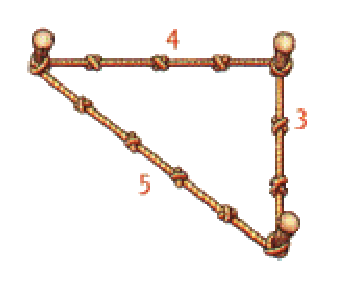
\includegraphics[width=3.5cm]{Geometrie/Images/G10_cours_corde}
\end{minipage}
\begin{minipage}{12cm}
  {\it Les géomètres égyptiens de l'époque pharaonique (donc bien avant la naissance de Pythagore) disposaient d'une corde sur laquelle ils avaient effectué 13 n\oe uds consécutifs situés à des intervalles réguliers. Celle-ci permettait de former des angles droits.}
\end{minipage}


%%%%%%%%%%%%%%%%%%%%%%%%%%%
\section{Trigonométrie dans le triangle rectangle}

\begin{definition}[Cosinus, sinus, tangente]
   Soit $ABC$ un triangle rectangle en $A$; on note $\alpha$ la mesure l'angle aigu $\widehat{ACB}$, on a :
   $$\cos \alpha=\dfrac{\text{côté adjacent}}{\text{hypoténuse}}=\dfrac{CA}{CB} \phantom{blanc} ; \qquad \sin \alpha=\dfrac{\text{côté opposé}}{\text{hypoténuse}}=\dfrac{BA}{BC}$$
   $$\tan \alpha=\dfrac{\text{côté opposé}}{\text{côté adjacent}}=\dfrac{AB}{AC}$$
\end{definition}

\begin{minipage}{9cm}
   \psset{unit=0.25}
   \begin{pspicture}(-14,-6)(14,12)
      \psline(-2.9,3.7)(4.23,7.57)
      \psline(4.23,7.57)(10.07,-3.27)
      \psline(10.07,-3.27)(-2.9,3.7)
      \rput{-62}(9,3.5){\textcolor{blue}{côté adjacent à l'angle $\alpha$}}
      \rput{29}(-0.5,7.5){\textcolor{blue}{côté opposé à l'angle $\alpha$}}
      \rput{-28}(2,-0.5){\textcolor{blue}{hypoténuse}}
      \rput(-3.5,3.7){$B$}
      \rput(4.3,8.5){$A$}
      \rput(10.5,-4){$C$}
      \psarc[linecolor=blue](10.07,-3.27){1.5}{120}{153}
      \psline(3.7,7.28)(4,6.73)
     \psline(4,6.73)(4.53,7.02)
      \rput(8.2,-1.3){\textcolor{blue}{\large$\alpha$}}
   \end{pspicture}
\end{minipage}
\begin{minipage}{4cm}
   exemple de moyen mnémotechnique pour se rappeler des formules : \\ [10pt]
   \hspace*{1cm} $\dfrac{\text{SO\,CA\,TO}}{\text{\phantom{S}H\,\phantom{C}H\,\phantom{T}A}}$
\end{minipage}

Ces formules permettent de calculer la mesure d'un angle dans un triangle rectangle.

\begin{exemple}
    Soit le triangle $ABC$ rectangle en $A$, avec $AB =\ucm{12}$ et $AC =\ucm{16}$. \\
    Calculer l'angle $\widehat{ACB}$.
   \correction
      On peut calculer la mesure de l'angle $\widehat{ACB}$ en utilisant la formule de la \textbf{tangente} : \\ [1mm]
      $\tan \widehat{ACB}=\dfrac{AB}{AC} =\dfrac{\ucm{12}}{\ucm{16}} =\dfrac34$ \\ [1mm]
      d'où $\widehat{ACB} =\arctan\left(\dfrac34\right) \simeq\udeg{36,9}$.
\end{exemple}

\begin{remarque}
   la touche 
\includegraphics[width=1cm]{Geometrie/Images/G10_cours_arctan} ou 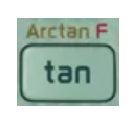
\includegraphics[width=1cm]{Geometrie/Images/G10_cours_tan}de la calculatrice permet de déterminer l'angle correspondant à une tangente.
\end{remarque}

\medskip

Inversement, les formules de trigonométrie permettent de calculer la longueur d'un côté dans un triangle rectangle.

\begin{exemple}
   Soit le triangle $ABC$ rectangle en $A$ tel que $AB =\ucm{12}$ et $\alpha =\widehat{ACB} =\udeg{30}$. \\
   Calculer BC.
   \correction
      On peut calculer la longueur du côté $[BC]$ en utilisant la formule du \textbf{sinus} : \\ [1mm]
      $\sin\alpha =\sin \widehat{ACB} =\dfrac{BA}{BC}$ \\ [1mm]
      d'où $BC =\dfrac{BA}{\sin \alpha} =\dfrac{\ucm{12}}{\sin\udeg{30}} =\ucm{24}$.
\end{exemple}

\begin{propriete}[Trigonométrie]
   Si $\alpha$ est la mesure (en degrés) d'un angle aigu dans un triangle. \\
   On a $0<\alpha<\udeg{90}$ et les propriétés suivantes :
   \begin{itemize}
      \item $0<\cos \alpha<1$ \quad et \quad $0<\sin \alpha<1.$
      \item $\cos^2\alpha+\sin^2\alpha=1$ \quad et \quad $\tan \alpha=\dfrac{\sin \alpha}{\cos \alpha}.$
   \end{itemize}
\end{propriete}


%%%%%%%%%%%%%%%%%%%%%%%%%%%%%%%
%%%%%%%%%%%%%%%%%%%%%%%%%%%%%%%
\activites


%%%
\begin{activite}[Groupement 1 - Exercice 5 - Question 2 : Pythagore]
   \ \\ [-16mm]
   \begin{QCM}
      \begin{minipage}{12cm}
         Un ballon-sonde est un ballon à gaz utilisé pour faire des mesures locales dans l'atmosphère. \\
         Dans le cadre du projet scientifique qu’elle anime pour sa classe de CM2, une professeure des écoles a reçu un petit ballon-sonde, représenté ci-contre. \\  
         Son enveloppe, composée de matières plastiques et de latex, a la forme, une fois gonflée, d'un cône de révolution surmonté d'une demi-sphère. \\ [3mm]
         Montrer qu’une génératrice du cône mesure $\sqrt{9000}$ cm. \\      
      \end{minipage}
      \qquad
      \begin{minipage}{5cm}
         {\psset{unit=0.5}
         \footnotesize
            \begin{pspicture}(-1,-1.5)(5,8)
               \psline(5,5.9)(3,0)(1,5.9)
               \psellipticarc(3,6)(2,0.7){180}{0}
               \psellipticarc[linestyle=dotted](3,6)(2,0.7){0}{180}
               \psarc(3,6){2}{0}{180}
               \psline[linestyle=dashed](3,0)(3,6)(5,6)
               \psframe(3,6)(3.2,5.8)
               \rput{-90}(3.3,3.1){90 cm}
               \rput(4,6.3){30 cm}
               \psarc(3,0){1.2}{70}{90}
               \rput(3.25,1.5){$\alpha$}
               \rput(3,-0.3){$S$}
               \rput(2.7,6.3){$O$}
               \rput(5.3,6){$N$}      
            \end{pspicture}}
      \end{minipage}
   \end{QCM}
   
   \bigskip
   
   \textcolor{G1}{
   {\bf Exemple de corrigé.} \\ \smallskip
      Dans le cône de révolution, $[SN]$ est une génératrice, et la hauteur $[OS]$ est perpendiculaire au rayon $[ON]$. \\
      On peut donc appliquer le théorème de Pythagore dans le triangle $SON$ rectangle en $O$ : \\
      $SN^2 =OS^2+ON^2 = (\ucm{90})^2+(\ucm{30})^2$ \\
      \hspace*{27mm} $ =\ucmq{8100}+\ucmq{900} =\ucmq{9000}$ \\
      \uline{La génératrice du cône mesure $\sqrt{9000}$ cm}.} \medskip
\end{activite}

\bigskip


%%%
\begin{activite}[Groupement 2 - Exercice 3 - Questions 1 et 2 : Pythagore et tracé]
   \ \\ [-16mm]
   \begin{QCM}
      \begin{minipage}{9cm}
         On considère un pavé droit $ABCDA’B’C’D’$ avec \\
         $DD’ =\ucm{5}$ ; $DC =\ucm{6}$ et $DA =\ucm{7}$. \\
         On note $L$ le point d’intersection des diagonales $[AC]$ et $[BD]$. \\
         On souhaite creuser ce pavé, en retirant une pyramide $OABCD$ de hauteur $[OL]$. \\
         Dans cette partie, on suppose que $OL =4$ cm.
         \begin{enumerate}
            \item Montrer que $AL\approx\ucm{4,6}$.
            \item Construire le triangle $ALO$ en vraie grandeur.
         \end{enumerate}
      \end{minipage}
      \begin{minipage}{7cm}
         \begin{pspicture}(-1,-1)(6,4.2)
         \psset{yunit=1.4}
            \pstGeonode[CurveType=polygon,PointSymbol=none,PosAngle={-135,-45,0,45,135,135},PointName={D',C',B',B,A,D}](0,0){D'}(4,0){C'}(5.5,0.7){B'}(5.5,2.7){R}(1.5,2.7){S}(0,2){D}
            \small
            \pstGeonode[PointSymbol=none,PosAngle={90,-90,135,90}](4,2){C}(2.75,1){O}(1.5,0.7){A'}(2.75,2.35){L}
            \pstLineAB{D}{C}
            \pstLineAB{C}{R}
            \pstLineAB{C}{C'}
            \psset{linestyle=dashed}
            \pstLineAB{D'}{A'}
            \pstLineAB{A'}{B'}
            \pstLineAB{S}{A'}
            \psset{linestyle=dotted}
            \pstLineAB{D}{R}
            \pstLineAB{S}{C}
            \pstLineAB{S}{O}
            \pstLineAB{R}{O}
            \pstLineAB{C}{O}
            \pstLineAB{D}{O}
            \pstLineAB{L}{O}
         \end{pspicture}
      \end{minipage} 
   \end{QCM}
   
   \bigskip
   
   \textcolor{G1}{
   {\bf Exemple de corrigé.} \smallskip
      \begin{enumerate}
         \item Dans le triangle $ADC$ rectangle en $D$, d'après le théorème de Pythagore, on a : \\ [1mm]
            $AC^2 =AD^2+DC^2 =(\ucm{7})^2+(\ucm{6})^2$ \\
            \hspace*{2.85cm} $=\ucmq{49}+\ucmq{36} =\ucmq{85}$, soit $AC =\sqrt{85}\,\ucm{}$. \\
            $L$ étant le point d'intersection des diagonales du rectangle $ABCD$, il est situé au milieu de chaque diagonale, donc $AL =\dfrac12AC =\dfrac12\sqrt{85}\ucm{} \approx\ucm{4,61}$. \uline{On a bien $AL \approx\ucm{4,61}$}. \smallskip
         \item $[OL]$ est la hauteur de la pyramide $OABCD$, on a donc $(OL)$ perpendiculaire au plan $(ABC)$, donc à toute droite de ce plan, en particulier à $(AL)$. \\
            Il suffit donc de tracer le triangle $ALO$ rectangle en $L$ tel que $OL =\ucm{4}$ et $AL \approx\ucm{4,61}$.
      \end{enumerate}}
\end{activite}

\pagebreak


%%%
\begin{activite}[Groupement 3 - Exercice 3 - Question 1 : Pythagore]
   \ \\ [-16mm]
   \begin{QCM}
      Une enseignante a le projet d’installer un potager \uline{rectangulaire} $ADEF$ sur une parcelle de forme triangulaire $ABC$ dans l’enceinte de l’école. \\
      Les points $A, B, C, D, E$ et $F$ sont tels que :
      \begin{itemize}
         \item $AB =\um{24}$, $AC =\um{10}$ et $BC =\um{26}$ ;
         \item $D\in[AB], E\in[BC]$ et $F\in[AC]$.
      \end{itemize}
      \begin{center}
         \small
         \psset{yunit=1.3}
            \begin{pspicture}(-1,-0.3)(12,5.5)     
               \rput{10}(0,0){\pstTriangle[PointSymbol=none,PointName={A,B,C}]{S}(12,0){R}(0,5){C}
               \psframe[fillstyle=vlines](0,0)(2,4.17)
               \rput(2,-0.3){$D$}
               \rput(-0.3,4.17){$F$}
               \rput(2.2,4.5){$E$}}
            \end{pspicture} \\
            {\it La figure ci-dessus n'est pas à l'échelle.} \smallskip
      \end{center}
      Montrer que le triangle $ABC$ est rectangle en $A$.
   \end{QCM}
   
   \bigskip
   
   \textcolor{G1}{
   {\bf Exemple de corrigé.} \\ [1mm]
      Dans le triangle $ABC$, on a d'une part : $BC^2 =(\um{26})^2 =\um{676}^2$ ; \\ [1mm]
      et d'autre part, $AB^2+AC^2 =(\um{24})^2+(\um{10})^2 =\um{576}^2+\um{100}^2 =\um{676}^2$. \\ [1mm]
      $BC^2 =AB^2+AC^2$, d'après la réciproque du théorème de Pythagore, \uline{le triangle $ABC$ est rectangle en $A$}.}
\end{activite}


%%%%%%%%%%%%%%%%%%%%%%%%%%%%%%%
%%%%%%%%%%%%%%%%%%%%%%%%%%%%%%%
\exercicesbase 

\begin{center}
   {\cursive Maîtriser les bases avec} \href{http://mathenpoche.sesamath.net}{
\includegraphics[width=3cm]{Nombres_et_calculs/Images/mathenpoche}} \\
   \bigskip
   {\hautab{0.85}
   \cursive
   \begin{Ltableau}{0.775\linewidth}{4}{C{1}|C{1}|p{7cm}|p{2.3cm}}
      \hline
      Classe & \texttt{N\degre} & Thème & Dans le cours \\
      \hline
      \textcolor{violet}{\bf 4\up{e}} & \texttt{D3} & Triangles rectangles & 1. et 2. \\
      \hline
      \textcolor{teal}{\bf 3\up{e}} & \texttt{D3} & Triangles rectangles & 3. \\
      \hline
   \end{Ltableau}}
\end{center}

\bigskip


\begin{exercice}[Pouce !] %%%1
   Marc décide de calculer la longueur de la diagonale de l'écran de sa console (écran rectangulaire). \\
   Il sait que cet écran mesure \ucm{5,2} de large et \ucm{6,2} de long.
   \begin{enumerate}
      \item Calculer la longueur de cette diagonale au millimètre près.
      \item Sur la publicité de cette console, il est indiqué que sa diagonale mesure trois pouces. En déduire une valeur approchée de un pouce.
      \item Un netbook a un écran de 10,1 pouces. Quelle est la longueur de la diagonale de l'écran de ce netbook en cm ?
   \end{enumerate}
\end{exercice}

\begin{corrige}
   On a la figure suivante : \\
   \begin{center}
   {\psset{unit=0.9}
      \begin{pspicture}(0,-0.5)(5,4.8)
         \pstGeonode[PosAngle={-135,-45,45,135},CurveType=polygon,PointSymbol=none](0,0){A}(6.2,0){B}(6.2,5.2){C}(0,5.2){D}
         \pstLineAB[linecolor=B1]{A}{C}
      \end{pspicture}}
   \end{center}
   \begin{enumerate}
      \item Le triangle ABC étant rectangle en B, on peut appliquer le théorème de Pythagore, avec des mesures en cm : \\
      $\text{AC}^2 =\text{AB}^2+\text{BC}^2 \iff \text{AC}^2 =6,2^2+5,2^2$ \\
      $\iff \text{AC}^2 =38,44+27,04 =65,48$ \\
      \; $\Longrightarrow \text{AC} =\sqrt{65,48} \approx8,09$. \\
      {\blue La diagonale de sa console mesure environ \ucm{8,1}.}
      \item 3 pouces correspondent à \ucm{8,1} ; donc, 1 pouce correspond à $\ucm{8,1}\div3 =\ucm{2,7}$. \\
      {\blue Un pouce vaut environ \ucm{2,7}.}
      \item $10,1\times2,7 = 27,27$ donc, {\blue la diagonale d'un netbook de 10,1 pouces est d'environ \ucm{27,3}.}
   \end{enumerate}
\end{corrige}

\bigskip


\begin{exercice}[Pêle-même] %%%2
\ \\ [-10mm]
  \begin{enumerate}
      \item ABC est un triangle rectangle en B tel que AB = \ucm{2,4} et $\widehat{\text{ACB}} =\udeg{44}$. Calculer AC au mm près.
      \item SRT est un triangle rectangle en S tel que SR = \ucm{4} et RT =\ucm{6}. Calculer la mesure de l'angle $\widehat{\text{SRT}}$.
      \item ATR est un triangle rectangle en A tel que AT = \ucm{9,6} et $\widehat{\text{TRA}} = \udeg{30}$. Calculer AR au mm près.
   \end{enumerate}
\end{exercice}

\begin{corrige}
\ \\ [-5mm]
   \begin{enumerate}
      \item On peut calculer $AC$ en utilisant la formule du \textbf{sinus} : \\ [1mm]
         $\sin\widehat{ACB}=\dfrac{AB}{AC}$ d'où $AC =\dfrac{\ucm{2,4}}{\sin \udeg{44}} \approx {\blue  \ucm{3,5}}$. \smallskip
      \item On peut calculer la mesure de l'angle $\widehat{SRT}$ en utilisant la formule du \textbf{cosinus} : \\ [1mm]
         $\cos \widehat{SRT}=\dfrac{RS}{RT} =\dfrac{\ucm{4}}{\ucm{6}} =\dfrac23$ d'où $\widehat{SRT} =\arccos\left(\dfrac23\right) \approx {\blue \udeg{48,2}}$. \smallskip
      \item On peut calculer $AR$ en utilisant la formule de la \textbf{tangente} : \\ [1mm]
         $\tan\widehat{ART}=\dfrac{AT}{AR}$ d'où $AR =\dfrac{\ucm{9,6}}{\tan \udeg{30}} \approx {\blue \ucm{16,6}}$.
   \end{enumerate}
\end{corrige}

\bigskip


\begin{exercice}[CRPE 2005 Besançon] %%%3
   Les nombres $a$, $b$ et $c$ sont des nombres entiers tels que $0 < a \leq b \leq c$. \\
   On suppose que $a$, $b$ et $c$ sont les mesures de longueur des côtés d'un triangle rectangle. \\
   Montrez que l'un au moins de ces trois nombres est pair.
\end{exercice}

\begin{corrige}
   {\bf Remarque initiale :} soit $N =2n+1$ un nombre impair, alors $N^2 =4n^2+4n+1$ est encore un nombre impair. \\
   Soit $N'=2n'+1$ un autre nombre impair, alors $N'^2 =4n'^2+4n'+1$ est un nombre impair. \\
   La somme $N+N'=4n^2+4n'^2+4n+4n'+2 =2(2n^2+2n'^2+2n+2n'+1)$ est un nombre pair. \\ [2mm]
   {\bf Démonstration :} on effectue une démonstration par l'absurde en supposant que la conclusion est fausse. Le contraire de \og l’un au moins de ces trois nombres est pair \fg{} est \og les trois nombres sont impairs \fg. \\
   Supposons alors que $a$, $b$ et $c$ soient tous les trois impairs, alors $a^2$, $b^2$ et $c^2$ le sont également. \\
   Or, le triangle dont les longueurs sont $a$, $b$ et $c$ est rectangle, donc $a^2 + b^2 = c^2$, ce qui signifie que $c^2$ est un nombre pair d'après la remarque initiale. L'hypothèse de départ est donc fausse : $a$, $b$ et $c$ ne peuvent pas être tous les trois impairs. D'où : {\blue l'un des trois nombres $a, b, c$ au moins est pair.}
\end{corrige}

\bigskip


\begin{exercice}[CRPE 2005 Grenoble] %%%4
   Le parallélépipède rectangle ABCDEFGH ci-dessous est coupé selon un plan et la section obtenue est le quadrilatère DPRH.
\begin{center}
   {\psset{xunit=1.4}
   \begin{pspicture}(0,-0.5)(5,4.3)
      \pspolygon(0,0)(4,0)(5,1)(5,4)(1,4)(0,3)
      \psline(0,3)(4,3)(4,0)
      \psline(4,3)(5,4)
      \psline[linestyle=dashed](0,0)(1,1)(5,1)
      \psline[linestyle=dashed](1,1)(1,4)
      \psline(4,3)(2,4)
      \psline[linestyle=dashed](2,4)(2,1)(4,0)
      \begin{small}
         \rput(0.8,4.3){B}
         \rput(2,4.3){P}
         \rput(1.8,0.8){R}
         \rput(-0.3,3){A}
         \rput(-0.3,-0.3){E}
         \rput(0.7,1.1){F}
         \rput(5.3,4.3){C}
         \rput(4.2,2.9){D}
         \rput(4.3,-0.3){H}
         \rput(5.3,0.9){G}
      \end{small}
   \end{pspicture}}
\end{center}
   On donne EH = \ucm{8}, HG = \ucm{5}, CG = \ucm{4} et BP = \ucm{2}.
   \begin{enumerate}
      \item Tracez en vraie grandeur le quadrilatère DPRH.
      \item Calculez la valeur exacte de PH.
      \item Calculez le volume du prisme ABPDEFRH.
   \end{enumerate}
\end{exercice}

\begin{corrige}
\ \\ [-5mm]
\begin{enumerate}
   \item Figure à l'échelle: \\
      \begin{pspicture}(-4.5,-3.5)(9,5)
         \pstGeonode[PosAngle={-135,-45,45,135},CurveType=polygon,PointSymbol=none](0,0){A}(8,0){D}(8,5){C}(0,5){B}
         \pstGeonode[PosAngle=90,PointSymbol=none](2,5){P}(-0.56,1.93){R}(5.44,-3.07){H}
         \pstLineAB[linecolor=B2]{P}{D}
         \pstLineAB[linecolor=B2]{P}{R}
         \pstLineAB[linecolor=B2]{R}{H}
         \pstLineAB[linecolor=B2]{H}{D}
         \pstRightAngle{P}{C}{D}
         \pstRightAngle[linecolor=G1]{P}{D}{H}
         \pstLineAB[linecolor=A1]{P}{H}
         \psarc[linecolor=B1](8,0){4}{210}{240}
      \end{pspicture}
   \item{\bf Calcul de DP :} dans le triangle DCP rectangle en C, on utilise le théorème de Pythagore avec des mesures en cm : $\text{DP}^2 =\text{DC}^2+\text{CP}^2 =5^2+(8-2)^2 =25+36 =61 \Longrightarrow \text{DP} =\sqrt{61}$ cm. \\ [1mm]
      {\bf Calcul de PH :} le triangle PDH est rectangle en H, d'après le théorème de Pythagore, on a \\
      $\text{PH}^2 =\text{PD}^2+\text{DH}^2 =61+16 =77 \Longrightarrow$ {\blue PH $=\sqrt{77}$ cm.}
   \item Le volume d'un prime se calcule en multipliant l'aire de sa base par sa hauteur. \\ [1mm]
   Calcul de l'aire de la base : $\mathcal{A} =\dfrac{(\text{BP}+\text{AD})\times\text{AB}}{2} =\dfrac{(\ucm{2}+\ucm{8})\times\ucm{5}}{2} =\ucmq{25}$ \\ [1.5mm]
   Calcul du volume du prisme : $\mathcal{V} =\mathcal{A}\times\text{AE} =\ucmq{25}\times\ucm{4} =\ucmc{100}$. \\ [1.5mm]
   {\blue Le volume du prisme ABPDEFRH est de \ucmc{100}.}
\end{enumerate}
\end{corrige}

\bigskip


\begin{exercice}[CRPE 2014 G2] %%%5
   Albert part dans les Alpes Autrichiennes, dans la station de ski de Kitzbühel. \\
   Lors de la montée à la station, sur le dernier tronçon de route montant à la station en ligne droite, Albert a vu un panneau signalant une pente constante de 25\,\%. La pente est le rapport entre le dénivelé et le déplacement horizontal (théorique). \\
   Ainsi une pente de 25\,\% indique un dénivelé de \um{25} pour un déplacement horizontal de \um{100}. \\   
   \begin{pspicture}(-1,-1)(8,4.5)
      \pspolygon(0,0)(5,0)(5,3)
      \rput(2.5,-0.5){déplacement horizontal}
      \rput(5.8,1.5){dénivelé}
      \rput(2,1.8){route}
   \end{pspicture}
   \begin{pspicture}(-1,-1)(8,4)
      \pspolygon(0,0)(5,0)(5,3.2)
      \rput(2.5,-0.5){100 m}
      \rput(5.6,1.5){25 m}
      \rput(2,1.8){route}
      \psarc(0,0){1}{0}{30}
      \rput(1.3,0.3){$\alpha$}
      \rput(2.5,3.5){\it La figure n'est pas à l'échelle}
   \end{pspicture} \\  
   On note $\alpha$ l'angle que la route forme avec l'horizontale. Cet angle est appelé l'inclinaison de la route.
   \begin{enumerate}
      \item Calculer, au degré près, l'inclinaison du dernier tronçon de la route empruntée par Albert.
      \item Ce tronçon de route permet de s'élever de \um{145}. Calculer sa longueur, au mètre près.
   \end{enumerate}
\end{exercice}

\begin{corrige}
\ \\ [-5mm]
   \begin{enumerate}
      \item On peut calculer la mesure de l'angle $\alpha$ en utilisant la formule de la tangente : \\ [1mm]
         $\tan \alpha =\dfrac{\um{25}}{\um{100}} =0,25$ d'où $\alpha =\arctan(0,25) \approx\udeg{14,04}$. \\ [1mm]
         {\blue L'inclinaison de la route est d'environ \udeg{14}}.
      \item On peut calculer la longueur $\ell$ de la route en utilisant la formule du sinus : \\ [1mm]
         $\sin\alpha =\dfrac{\um{145}}{\ell}$ d'où $\ell =\dfrac{\um{145}}{\sin \udeg{14}} \approx \um{599,4}$. \\ [1mm]
         {\blue La route mesure environ \um{599}.}
   \end{enumerate}
\end{corrige}

\bigskip


\begin{exercice}[CRPE 2016 G3] %%%6
   On donne trois points A, B, C tels que AB = \ucm{8}, AC = \ucm{6} ; les droites (AB) et (AC) sont perpendiculaires. \\  
   On place :
   \begin{itemize}
      \item un point D appartenant au segment [AB] distinct de A et B ;
      \item le point E, intersection du segment [BC] et de la perpendiculaire à la droite (AB) passant par D ;
      \item le point F, intersection du segment [AC] et de la perpendiculaire à la droite (AC) passant par E.
   \end{itemize}
   \begin{center}
      {\psset{unit=1.3}
      \begin{pspicture}(0,-0.3)(4,3.5)
         \psline(0,3)(0,2.2)(1,0)(4,0)
         \psframe[linestyle=dashed](0,0)(1,2.2)
         \psline[linestyle=dashed](0,3)(4,0)
         \psframe(0,0)(0.2,0.2)
         \psframe(1,0)(1.2,0.2)
         \psframe(0,2)(0.2,2.2)
         \rput(-0.2,-0.2){\small A}
         \rput(1,-0.3){\small D}
         \rput(4.2,-0.2){\small B}
         \rput(-0.2,2.2){\small F}
         \rput(-0.2,3.2){\small C}
         \rput(1.2,2.4){\small E}
      \end{pspicture}
      }
   \end{center}
   \begin{enumerate}
      \item Démontrer que BC = \ucm{10}.
      \item Déterminer une mesure en degré de l’angle $\widehat{ABC}$ (on donnera le résultat arrondi à l’unité).
      \item Démontrer que AE = DF.
   \end{enumerate}
\end{exercice}

\begin{corrige}
\ \\ [-5mm]
   \begin{enumerate}
      \item Dans le triangle ABC rectangle en A, on applique le théorème de Pythagore avec des mesures en cm : \\
         $\text{BC}^2=\text{BA}^2+\text{AC}^2 =8^2+6^2 =64+36 =100 \Longrightarrow {\blue BC = \ucm{10}}$.   
   \item Dans le triangle ABC rectangle en A, on utilise le cosinus : \\ [1mm]
      $\cos(\widehat{ABC}) =\dfrac{BA}{BC} =\dfrac{8}{10} =\dfrac45 \Longrightarrow \widehat{ABC} =\arccos\left(\dfrac45\right) \approx {\blue \udeg{37}}$. \smallskip
   \item Le quadrilatère ADEF possède trois angles droits, c'est donc un rectangle. Or, les diagonales d'un rectangle sont de même longueur d'où :
      {\blue AE = DF}.
   \end{enumerate}
\end{corrige}

\bigskip


\begin{exercice}[CRPE 2009 G1] %%%%%%%%%%%%%%%%%%
   On considère deux points A et B du plan distants de \ucm{6}.
   \begin{enumerate}
      \item 
         \begin{enumerate}
            \item Le point C$_1$ est sur le segment [AB] et vérifie la condition BC$_1$= 2 AC$_1$. Quelle est la longueur du segment [AC$_1$] ? Justifier.
            \item Le point C$_2$, distinct de C$_1$, est sur la droite (AB) et vérifie la condition BC$_2$ = 2 AC$_2$. Quelle est la longueur du segment [AC$_2$] ? Justifier.
            \item Placer, avec une règle graduée, les points A, B, C$_1$ et C$_2$ sur une figure qui sera complétée au fur et à mesure des questions. 
         \end{enumerate}       
      \item On s'intéresse maintenant aux points C du plan n'appartenant pas à la droite (AB) et vérifiant la condition BC~=~2AC. On appelle $x$ la mesure de AC, l'unité de longueur étant le centimètre.
         \begin{enumerate}
            \item Existe-t-il des points C correspondant à la valeur $x=9$ ? Justifier la réponse. Dans le cas d'une réponse positive, construire ces points.
            \item Existe-t-il des points C correspondant à la valeur $x=5$ ? Justifier la réponse. Dans le cas d'une réponse positive, construire ces points.
         \end{enumerate}
      \item Calculer la valeur de $x$ pour laquelle le triangle ABC est rectangle en C. Ecrire le résultat sous la forme $a\sqrt5$ .
      \item Montrer qu'il existe une seule valeur de $x$ pour laquelle le triangle ABC est isocèle. Déterminer cette valeur et placer les points correspondants sur la figure en laissant apparents les tracés nécessaires à cette construction.
   \end{enumerate}
\end{exercice}

\begin{corrige}
\ \\ [-5mm]
   \begin{enumerate}
      \item 
         \begin{enumerate}
            \item le point C$_1$ est sur le segment [AB], donc entre A et B. On a alors : BC$_1$ = BA $-$ AC$_1$. \\
               D'où les équivalences : BC$_1$ = 2AC$_1 \iff$ BA $-$ AC$_1$ = 2AC$_1 \iff$ BA = 3AC$_1 \iff$ AC$_1 = \dfrac13$ AB. \\
               Or, AB = \ucm{6}, donc : {\blue la longueur du segment [AC$_1$] est de \ucm{2}}.
         \item Si BC$_2$ = 2 AC$_2$ et C$_2$ distinct de C$_1$, alors BC$2$ est plus grand que AC$_2$ et donc le point C$_2$ est en dehors du segment [AB], du côté de A. On a alors : BC$_2$ = BA + AC$_2$. D'où les équivalences : \\
            BC$_2$ = 2AC$_2 \iff$ BA + AC$_2$ = 2AC$_2 \iff$ BA = AC$_2$. \\
            Donc : {\blue la longueur du segment [AC$_2$] est de \ucm{6}}.
         \item Une figure possible : \\
            {\psset{unit=0.7}
            \begin{pspicture}(-3,-6.2)(16,6.2)
               \psgrid[subgriddiv=10, gridlabels=0, gridwidth=0.4pt, subgridwidth=0.4pt,gridcolor=brown!80,subgridcolor=brown!40](-1,-6)(16,6)
               \psline(-1,0)(16,0)
               \psline[linewidth=0.05cm](6,0)(12,0)
               \psline[linewidth=0.05cm](6,0)(6.75,2.9)(12,0)
               \psline[linewidth=0.05cm](6,0)(6.75,-2.9)(12,0)
               \psdots(6,0)(12,0)(0,0)(8,0)
               \psdots[linecolor=A1](6.75,-2.9)(6.75,2.9)
               \psdots[linecolor=B2](2.75,3.8)(2.75,-3.8)
               \pscircle[linecolor=B2](6,0){5}
               \psarc[linecolor=B2](12,0){10}{143}{-143}
               \pscircle[linecolor=A1](6,0){3}
               \psarc[linecolor=A1](12,0){6}{48}{-48}
               \rput[bl](6.1,0.3){A}
               \rput[bl](12,0.3){B}
               \rput[bl](8,0.3){C$_1$}
               \rput[bl](0,0.3){C$_2$}
               \rput[bl](2,4){\textcolor{B2}{$C_3$}}
               \rput[bl](2,-4.4){\textcolor{B2}{$C_4$}}
               \rput[bl](6.3,-3.7){\textcolor{A1}{$C_6$}}
               \rput[bl](6.3,3.4){\textcolor{A1}{$C_5$}}
            \end{pspicture}}
         \end{enumerate} 
      \setcounter{enumi}{1}
      \item Si AC $=x$, alors BC $=2x$. De plus, si C existe, A, B et C ne sont pas alignés et forment donc un triangle.
         \begin{enumerate}
            \item Si $x=9$, alors AC = \ucm{9} et BC = \ucm{18}. Or, AB = \ucm{6}, et $6+9 =15$ donc, BA + AC < BC, ce qui signifie qu'on ne peut pas construire un triangle. \\
            {\blue Il n'existe pas de point C pour $x=9$}.
            \item Si $x=5$, alors AC = \ucm{5} et BC = \ucm{10}. Or, AB = \ucm{6}, et $6+5 =11$ donc, BA + AC > BC, ce qui signifie que l'on peut construire un triangle. Dans ce cas, C est sur le cercle de centre A de rayon \ucm{5} et sur le cercle de centre B de rayon \ucm{10}. Ces deux cercles sont sécants en deux points C$_3$ et C$_4$. \\
            {\blue Il existe deux points C pour $x=5$}.
         \end{enumerate}
      \setcounter{enumi}{2}
      \item D'après le théorème de Pythagore, dans le triangle ABC rectangle en C, on a : \\
         $\text{AB}^2 =\text{AC}^2+\text{BC}^2 \iff 6^2 =x^2+(2x)^2 \iff 36 =5x^2 \iff x^2 =\dfrac{36}{5} \Longrightarrow x=\dfrac{6}{\sqrt5} =\dfrac{6}{5}\sqrt5$. \\
         {\blue Pour $x=\dfrac65\sqrt5$, le triangle ABC est rectangle en C}. \smallskip
       \item Vérifions les cas où le triangle peut-être isocèle :
          \begin{itemize}
            \item Supposons qu'il soit isocèle en C, alors AC = BC $\iff x =2x \iff x=0$, ce qui est impossible.
            \item Supposons qu'il soit isocèle en A, alors CA = BA = \ucm{6} et BC = \ucm{12}. \\
               Mais dans ce cas, BA + AC = BC, donc A, B et C sont alignés, ce qui est contraire à l'énoncé.
             \item Supposons qu'il soit isocèle en B, alors AB = CB = \ucm{6} et AC = \ucm{3}. \\
               Dans ce cas, BA + AC > BC, donc, il existe deux points C$_5$ et C$_6$ tels que le triangle ABC soit isocèle en B.             
          \end{itemize}
         {\blue Il existe une seule valeur de $x$ (qui vaut 3) pour laquelle le triangle ABC est isocèle}.
   \end{enumerate}
\end{corrige}

\bigskip


\begin{exercice}[CRPE 2022 - Sujet 0] %%%9
   \begin{minipage}{9cm}
      On propose un jeu dans une cour de récréation. Pour cela on s’appuie sur des croix peintes au sol comme indiquée sur le schéma ci-contre :
      \begin{itemize}
         \item la croix $M$ est située à \um{30} du mur d’enceinte de l’école ($MR =\um{30}$) ;
         \item la croix $L$ est située à \um{40} du mur d’enceinte de l’école ($LS =\um{40}$) ;
         \item les points $R$ et $S$ sont distants de \um{50} ($RS =\um{50}$).
      \end{itemize}
   \end{minipage}
   \begin{minipage}{7cm}
      {\small
      \begin{pspicture}(-2.5,-1)(4.5,5)
         \psline(0,-0.5)(0,5.5)
         \psline[linestyle=dashed]{-|}(0,0)(4,0)
         \psline[linestyle=dashed]{|-|}(0,5)(3,5)
         \psframe(0,0)(0.3,0.3)
         \psframe(0,5)(0.3,4.7)
         \rput(-0.3,0){$S$}
         \rput(4.3,0){$L$}
         \rput(-0.3,5){$R$}
         \rput(3.3,5){$M$}
         \rput{-90}(0.3,2.5){Mur}
         \psline{<->}(-0.6,0)(-0.6,5)
         \rput(-1.1,2.5){\um{50}}
         \rput(2,0.3){\um{40}}
         \rput(1.5,5.3){\um{30}}
      \end{pspicture}}
   \end{minipage} \\
   Mila, une élève, se trouve sur la croix $M$ et Lucien, un autre élève, se trouve sur la croix $L$. L’enseignante souhaite que Mila et Lucien courent tous les deux vers un même point de contact au mur ; le gagnant sera le premier à toucher ce point sur le mur. Pour que l’épreuve soit équitable, l’enseignante souhaite que le point de contact soit à égale distance des positions initiales des deux élèves, c’est-à-dire des croix $L$ et $M$.
   \begin{enumerate}
      \item Construire à l’échelle le plan de la cour avec les points $M, L, R$ et $S$ en choisissant comme échelle \ucm{1} pour \um{5}.
      \item
      \begin{enumerate}
         \item Sur la figure, construire le point $T$, milieu du segment $[ML]$. Tracer la droite perpendiculaire à $(ML)$ et passant par $T$. On note $C$ le point d’intersection de cette droite avec le mur.
         \item Justifier que le point $C$ est le point de contact cherché.
         \item Mesurer la longueur $RC$ sur le plan et en déduire une estimation de la distance entre les points $R$ et $C$ dans la cour de récréation.
      \end{enumerate}
      \item On note $x$ la distance, exprimée en mètre, entre les points $R$ et $C$ dans la cour de récréation.
      \begin{enumerate}
         \item Déterminer les longueurs $MC$ et $CL$ en fonction de $x$.
         \item En déduire la distance entre les points $R$ et $C$ dans la cour de récréation.
      \end{enumerate}
   \end{enumerate}
\end{exercice}

\begin{corrige}
\ \\ [-5mm]
   \begin{enumerate}
      \item À l'échelle \ucm{1} pour \um{5}, \um{30}, \um{40} et \um{50} sont représentés par des segments de longueurs respectives \ucm{6}, \ucm{8} et \ucm{10}. \\
      {\psset{unit=2}
         \begin{pspicture}(-2,-0.25)(5,5.25)
            \pstGeonode[CurveType=polygon,PointSymbol=none,PosAngle={0,180,180,0},](4,0){L}(0,0){S}(0,5){R}(3,5){M}
            \pstRightAngle{L}{S}{R}
            \pstRightAngle{S}{R}{M}
            \rput{-90}(0.2,2.5){Mur}
            \pstMiddleAB[PosAngle=45]{M}{L}{T}
            \pstMediatorAB[CodeFig=true,CodeFigColor=black,PointSymbol=none,PointName=none,linestyle=dashed,nodesep=-1]{L}{M}{A}{B}
            \pstInterLL[PosAngle=180]{T}{B}{R}{S}{C}        
         \end{pspicture}}
      \item
      \begin{enumerate}
         \item Voir figure.
	      \item Le point $C$ appartient à la droite perpendiculaire au segment $[ML]$ passant par son milieu $T$, il appartient donc à la médiatrice de $[ML]$ et est situé à égale distance de $M$ et de $L$. \\
	         Par conséquent, {\blue $C$ est le point de contact cherché}.
	      \item On mesure la longueur demandée, on obtient $RC \approx\ucm{6,4}$ sur le plan. Or, $6,4\times5 =32$ donc, \\
	      {\blue la distance entre les points $R$ et $C$ dans le cour est de \um{32}}.
      \end{enumerate}
      \setcounter{enumi}{2}
      \item
      \begin{enumerate}
         \item $\bullet$ Dans le triangle $CRM$ rectangle en $R$, on utilise le théorème de Pythagore avec des mesures en mètre : \\
            $MC^2 =MR^2+RC^2 =30^2+x^2$ \\
            \hspace*{2.9cm} $=x^2+900$. \\
            $\bullet$ Dans le triangle $CSL$ rectangle en $S$, on utilise le théorème de Pythagore avec des mesures en mètre : \\
            $LC^2 =LS^2+SC^2 =40^2+(50-x)^2$ \\
            \hspace*{2.53cm} $=1\,600+(2\,500-100x+x^2)$ \\
            \hspace*{2.53cm} $=x^2-100x+4\,100$. \\ [1mm]
            On a donc {\blue $MC =\sqrt{x^2+900}$ et $LC =\sqrt{x^2-100x+4\,100}$}.
         \item Le point $C$ est à égale distance de $M$ et de $L$, on a donc $MC =CL$, on encore $MC^2 =CL^2$. \\
            $\cancel{x^2}+900 =\cancel{x^2}-100x+4\,100 \iff 100x =4\,100-900 =3\,200$ \\
            \hspace*{4.15cm} $\iff x =32$ \\
            {\blue On retrouve bien une distance de \um{32} entre les points $R$ et $C$}.
      \end{enumerate}
   \end{enumerate}
\end{corrige}

\bigskip


\begin{exercice}[CRPE 2019 G3] %%%8
   On considère la figure ci-dessous qui n’est pas représentée à l’échelle et qui vérifie les propriétés suivantes : \\
   \begin{minipage}{9cm}
      \begin{itemize}
         \item $BC =\ucm{8}$ ;
         \item $AB =\ucm{6}$ ;
         \item $AC =\ucm{10}$ ;
         \item $AD =\ucm{8}$ ;
         \item $D$ appartient aux segments $[AE]$ et $[BC]$ ;
         \item Les droites $(BC)$ et $(CE)$ sont perpendiculaires.
      \end{itemize}
   \end{minipage}
   \begin{minipage}{7cm}
      \begin{pspicture}(-0.5,0.2)(6.5,3.3)
         {\small
            \pstGeonode[CurveType=polygon,PosAngle={170,-90,45,-45,90},PointSymbol=none](0,3){A}(1,0){B}(5.5,1.5){C}(6,0){E}(4,1){D}
            \pstLineAB{A}{C}
            \pstRightAngle{D}{C}{E}
         }
      \end{pspicture}
   \end{minipage} \\
   Le but de l’exercice est de déterminer l’aire du triangle $ACE$.
   \begin{enumerate}
      \item Montrer que les droites $(AB)$ et $(BC)$ sont perpendiculaires.
      \item En déduire la longueur $BD$.
      \item Déterminer la longueur $CE$.
      \item Déterminer l’aire du triangle $ACE$.
   \end{enumerate}
\end{exercice}

\begin{corrige}
   Dans tout l'exercice, les longueurs sont exprimées en \ucm{} et les aires en \ucmq{}. \\
   \begin{enumerate}
      \item Dans le triangle $ABC$, on a d'une part : $AB^2+BC^2 =6^2+8^2 =36+64 =100$ \\
         et d'autre part : $AC^2 =10^2 =100$. \\
         On a alors $AB^2+BC^2 =AC^2$, et d'après la réciproque du théorème de Pythagore, on peut affirmer que le triangle $ABC$ est rectangle en $B$. \\
         Par conséquent, {\blue les droites $(AB)$ et $(BC)$ sont perpendiculaires}.
      \item Dans le triangle $ABD$ rectangle en $B$, on applique le théorème de Pythagore : \\
         $AD^2 =AB^2+BD^2 \iff 8^2 =6^2+BD^2$. \\
         D'où : $BD^2 =64-36 =28 \Longrightarrow BD =\sqrt{28} =2\sqrt7 \approx5,2915$. \\
         Conclusion : {\blue la longueur $BD$ vaut exactement $2\sqrt7\ucm{}$, soit approximativement \ucm{5,3}}.
      \item Les droites $(AB)$ et $(CE)$ dont toutes les deux perpendiculaires à la droite $(BC)$, elles sont donc parallèles entre elles. On a alors : $B, D, C$ et $A, D, E$ alignés dans cet ordre ; les droites $(AB)$ et $(CE)$ sont parallèle. \\ [1mm]
         D'après le théorème de Thalès et sa conséquence, $\dfrac{DC}{DB} =\dfrac{DE}{DA} =\dfrac{CE}{BA} \iff \dfrac{8-2\sqrt7}{2\sqrt7} =\dfrac{DE}{8} =\dfrac{CE}{6}$. \\
         On cherche $CE$ : $CE =\dfrac{6\times(8-2\sqrt7)}{2\sqrt7} \approx3,071$. {\blue La longueur $CE$ vaut environ \ucm{3,1}}. \smallskip
      \item Si on choisit $[CE]$ comme base du triangle $ACE$, alors sa hauteur associée est $[BC]$. \\ [1mm]
         On a alors : $\mathcal{A}(ACE) =\dfrac{CE\times BC}{2} \approx\dfrac{3,071\times8}{2} \approx12,284$. {\blue L'aire du triangle $ACE$ vaut environ \ucmc{12,3}}.
   \end{enumerate}
\end{corrige}

\bigskip


\begin{exercice}[CRPE 2017 G3] %%%10
   Un pont a une arche en forme d’arc de cercle. \\
   \begin{minipage}{6cm}
     Lors d’une crue, l’eau atteint les sommets A et B des piliers du pont. \\
     La hauteur maximale IC entre le niveau de l’eau et le sommet de l’arche est alors de 5 mètres. \\
     L'écartement AB entre les deux piliers du pont est de 24 mètres. \\
     La situation est modélisée par le schéma ci-contre, qui n’est pas à l’échelle, sur lequel O est le centre de l’arc de cercle $\wideparen{\text{AB}}$ et (CO) est l’axe de symétrie de la figure. 
   \end{minipage}
   \qquad
   \begin{minipage}{9cm}
      \begin{pspicture}(-1.5,-1)(8,7)
         \small
         \psline(0,0)(0,4)(8,4)(8,0)
         \psline(4,0)(4,7)
         \psline[linestyle=dashed](4,1)(0,4)
         \psarc(4,1){5}{37}{143}
         \rput(4.3,1){O}
         \rput(4.3,3.7){I}
         \rput(4.3,6.3){C}
         \rput(8.3,4.3){B}
         \rput(-0.3,4.4){A}
         \psline{->}(1,6)(1.5,4)
         \rput(1,6.3){niveau de l'eau}
         \psline{->}(6.8,7)(6,5.55)
         \rput(6.8,7.3){arche du pont}
      \end{pspicture}
   \end{minipage}
   \begin{enumerate}
      \item Montrer que le rayon OA de l’arche est 16,9 m.
      \item On assimile la coupe de la partie émergée d’une péniche, vue de face, à un rectangle de 4 mètres de haut et de 12 mètres de large. \\
      {\psset{unit=0.8}
      \begin{pspicture}(-3,-1)(12,3)
         \psline(0,0)(12,0)
         \psframe[fillstyle=solid,fillcolor=lightgray](2,0)(8,2)
         \rput(5,1){\large Péniche}
         \rput(1.7,-0.3){E}
         \rput(8.3,-0.3){H}
         \rput(1.7,2.3){F}
         \rput(8.3,2.3){G}
         \psline{->}(10.5,0.7)(10,0)
         \rput(10.5,1){Surface de l'eau}
      \end{pspicture}} \\
      La situation est modélisée par le schéma ci-dessus, qui n’est pas à l’échelle sur lequel on a EH = \um{12} et FE~= \um{4}. Cette péniche peut-elle passer sous l’arche du pont sans dommages ? Justifier.
   \end{enumerate}
\end{exercice}

\begin{corrige}
\ \\ [-5mm]
   \begin{enumerate}
      \item On considère le triangle AOI rectangle en I et on pose OA = OC = $x$. On a alors OI = $x-5$. \\
         On applique le théorème de Pythagore dans ce triangle avec des mesures en mètre. \\
         AO$^2$ = AI$^2$ + IO$^2 \iff x^2 = 12^2+(x-5)^2$ \\
         \hspace*{2.45cm} $\iff \cancel{x^2} =144+ \cancel{x^2}-10x+25$ \\
         \hspace*{2.45cm} $\iff 10x =169$ \\
         \hspace*{2.45cm}  $\iff x =16,9$. {\blue Le rayon OA de l'arche est \um{16,9}}.
      \item On considère le schéma de coupe suivant dans lequel on a représenté la moitié de la figure puisqu'il y a symétrie par rapport à (CO). Pour maximiser ses chances de passer sous l'arche, la péniche doit être centrée. \\
         \begin{minipage}{7cm}
         {\psset{unit=0.4}
         \small
            \begin{pspicture}(-1,-1.5)(14,18)
               \pspolygon(0,11.9)(12,11.9)(12,0)
               \psframe(12,15.9)(11.7,15.6)
               \psline(12,11.9)(12,16.9)
               \psarc(12,0){16.9}{90}{135.2}
               \psframe[fillstyle=solid,fillcolor=lightgray!50](6,11.9)(12,15.9)
               \psline(12,0)(6,15.9)
               \rput(9,14.3){Demi}
               \rput(9,13.6){Péniche}
               \rput(12,-0.5){O}
               \rput(6,16.5){F}
               \rput(12.5,15.9){J}
               \rput(12.5,11.9){I}
               \rput(12.5,17.4){C}
               \rput(-0.5,11.9){A}
               \rput(4.7,6){16,9 m}
               \rput(9.6,16.35){6 m}
               \rput(12.8,13.9){4 m}  
            \end{pspicture}}
         \end{minipage}
         \qquad
         \begin{minipage}{8cm}
            Pour savoir si la péniche passe sous l'arche, il faut vérifier que la distance OF (F étant le coin supérieur gauche de la péniche vue de face) est inférieure au rayon de l'arche (\um{16,9}). \\ [2mm]
            On a : OJ = OI + IJ \\
            \hspace*{1.35cm} = (OC $-$ IC) + IJ \\
            \hspace*{1.35cm} = ($\um{16,9}-\um{5}$) + \um{4} \\
            \hspace*{1.35cm} = \um{15,9}. \\ [2mm]
            Dans le triangle OJF rectangle en J, on utilise le théorème de Pythagore avec des mesures en mètre : \\
            $\text{OF}^2 = \text{OJ}^2 + \text{JF}^2$ \\
            \hspace*{0.65cm}  $= 15,9^2 + 6^2$ \\
            \hspace*{0.65cm}  $= 288,81$ \\
            Donc, OF $\approx$ \um{16,99} > \um{16,9}.
         \end{minipage}
      {\blue Cette péniche ne pourra pas passer sous l'arche sans dommage}.
   \end{enumerate}
\end{corrige}


%\begin{exercice}[Rectangle ou non ?] %%%1
%   On considère le triangle ABC ci-dessous (la figure n'est pas à l'échelle).
%   \begin{center}
%      \begin{pspicture}(-1,-1)(6,4)
%      {\psset{unit=1.2}
%         \pspolygon(0,0)(5,0)(1.5,2.5)
%         \psline(1.5,0)(1.5,2.5)
%         \psframe(1.5,0)(1.7,0.2)
%         \rput(0.2,1.5){\ucm{5}}
%         \rput(0.75,-0.4){\ucm{3}}
%         \rput(3,-0.4){\ucm{7}}
%         \rput(-0.3,-0.3){B}
%         \rput(5.3,-0.3){C}
%         \rput(1.5,2.8){A}
%         \rput(1.2,0.3){H}
%         \psline{<->}(0,-0.2)(1.5,-0.2)
%         \psline{<->}(1.5,-0.2)(5,-0.2)
%         \psline{<->}(-0.2,0)(1.3,2.5)}
%      \end{pspicture}
%   \end{center}
%   \begin{enumerate}
%      \item Calculer la hauteur AH.
%      \item Calculer la valeur arrondie au millimètre de la longueur du côté [AC].
%      \item Le triangle ABC est-il rectangle ?
%   \end{enumerate}
%\end{exercice}
%
%\begin{corrige}
%\ \\ [-5mm]
%\begin{enumerate}
%   \item Dans le triangle AHB rectangle en H, d'après le théorème de Pythagore, on a : \\
%   $\text{AB}^2 =\text{AH}^2+\text{HB}^2 \iff 5^2 =\text{AH}^2+3^2 \iff\text{AH}^2 =25-9 =16\Longrightarrow \text{AH} =\sqrt{16} =4$. \\
%   {\blue La hauteur AH mesure \ucm{4}.}
%   \item Dans le triangle AHC rectangle en H, d'après le théorème de Pythagore, on a : \\
%   $\text{AC}^2 =\text{AH}^2+\text{HC}^2 \iff \text{AC}^2 =4^2+7^2\iff\text{AC}^2 =16+49 =65\Longrightarrow \text{AC} =\sqrt{65}$. \\
%   {\blue Le côté AC mesure environ \ucm{8,1}.}
%\end{enumerate}
%\end{corrige}


%\begin{exercice}[CRPE 2012 G1] %%%5
%   La figure ci-dessous représente trois carrés construits sur les trois côtés d'un triangle rectangle. Dans chacun des carrés est indiquée son aire. \\
%   L'affirmation suivante est-elle vraie : la construction à l'échelle de cette figure est possible. \\
%   \begin{center}
%   {\psset{unit=0.7}
%   \rotatebox{-53}{
%      \begin{pspicture}(-4,-2)(8,0)
%         \pspolygon(0,-5)(5,-5)(5,0)(0,0)
%         \pspolygon(0,0)(1.8,2.4)(-0.6,4.2)(-2.4,1.8)
%         \pspolygon(1.8,2.4)(5,0)(7.4,3.2)(4.2,5.6)
%         \pspolygon(1.8,2.4)(1.6,2.13)(1.85,1.95)(2.05,2.2)
%         \rput(2.5,-2.5){\rotatebox{53}{\ucmq{100}}}
%         \rput(-0.3,2.1){\rotatebox{53}{\ucmq{32}}}
%         \rput(4.6,2.8){\rotatebox{53}{\ucmq{64}}}
%      \end{pspicture}}}
%   \end{center}
%\end{exercice}
%
%\begin{corrige}
%   Le carré d'aire 32 cm$^2$ a ses côtés de longueur $\sqrt{32}$ cm ; le carré d'aire 64 cm$^2$ a ses côtés de longueur $\sqrt{64}$ cm et le carré d'aire 100 cm$^2$ a ses côtés de longueur $\sqrt{100}$ cm. \\
%Or, $\sqrt{32}^2+\sqrt{64}^2 =32+64 = 96$ et $\sqrt{100}^2 =100 \not=96$. \\
%D'après le théorème de Pythagore, si le triangle était rectangle, on aurait l'égalité. Ce n'est pas le cas, il n'y a donc pas d'angle droit et {\blue il n'est pas possible de construire cette figure \og à l'échelle \fg.} \\
%\end{corrige}

